\documentclass{article} %[twocolumn] 

%\usepackage{algorithmic}
\usepackage{algorithm}
\usepackage{algorithmicx}
\usepackage{algpseudocode}
\usepackage{booktabs}
\usepackage{array}
\usepackage{graphicx}
\usepackage{amsmath}
\usepackage{amsfonts}
\usepackage{amssymb}

\title{Efficient and flexible simulation-based design of complex clinical trials}
\date{}

\begin{document}
0968979556
\maketitle

\begin{abstract}
[NOTE - COPY OF SCT / ICTMC ABSTRACT, TO REVISE] \textbf{Background}: Finding the optimal sample size for a trial is an important step in its design. In many trials of complex interventions (such as psychotherapies and behavioural interventions) this task is complicated by two factors. Firstly, sample size can be defined by several design parameters rather than a single n. For example, the TIGA-CUB trial compares a psychotherapy intervention with treatment as usual. The design is partially nested, with patients are nested within therapists in the intervention arm but not in the control arm. The design parameters are the number of therapists in the intervention arm, the number of patients seen by each therapist, and the number of patients in the control arm. The second complication is that analytical formulae for calculating power are not always available. As a result power must instead be estimated through Monte Carlo simulation methods, which may be computationally demanding. For example, such a simulation of the TIGA-CUB study would involve the generation of a large number of hypothetical trial data sets and fitting a multilevel model to each one. In combination, these factors make finding an optimal sample size a difficult and time consuming problem. We explore how modern optimisation algorithms can be used to solve these problems in an effective, timely manner.

\textbf{Methods}: We propose using Bayesian optimisation to solve the sample size problem. This method allows optimal or near-optimal choices for sample size to be found with minimal computational effort. The general approach involves the careful choice of the design parameter values where power should be estimated using simulation. Conducting the simulations at these points, a statistical model is then fitted to the output to describe the general relationship between the design parameters and the trial power. This model is then used to find the smallest design parameter values which will give power of at least the nominal level. The method is flexible, can be used for almost any problem for which power can be estimated using Monte Carlo simulation, and can be implemented using existing statistical software packages.

\textbf{Evaluation}: To illustrate the approach we apply it to the TIGA-CUB trial in an illustrative case study. We use the proposed method to identify a set of candidate sample size options, each of which will give power of at least the nominal rate. From this set of options, that which is considered best in terms of its balance between number of therapists and number of patients can be chosen. We compare this with an alternative approach using simpler heuristics, in terms of both the computation time required and the quality of the resulting solutions.

\textbf{Conclusions}: Bayesian optimisation can be an effective technique for performing sample size calculations when power must be estimated using simulation, particularly when sample size is characterised by several design parameters. By improving the efficiency of these calculations, increasingly complex sample size problems can be solved without the need for unrealistic simplifying assumptions.
\end{abstract}

\section{Introduction}\label{sec:intro}

Include:

\cite{Reich2012} - Empirical Power and Sample Size Calculations for Cluster-Randomized and Cluster-Randomized Crossover Studies
Proposes to use simulation for estimating power in cluster-randomised crossover studies. Doesn't explicitly consider methodology for SSD using these estimates, and in the examples only considers problems with a single design variables. Simulation function is in R, not C++ - and uses a for loop! Not much use.

\cite{Sutton2007} - Evidence-based sample size calculations based upon updated meta-analysis. Simulation approach, ``Although for simple situations closed form solutions are often possible,for more complex analyses, including those that include random effects, closed form solutionsoften do not exist and simulation methods become an appealing alternative''. Refers to~\cite{Feiveson2002} for a general guide. Later argues that even if closed form solutions could be derived, the flexibility of the simulation approach is preferable.

%When designing a clinical trial to test a hypothesis it is typical to choose the smallest sample size which will ensure the power of the trial is above some nominal threshold. When analytical formulae for calculating power are available, the computations required to determine this sample size can be carried out quickly. However, such power formulae are not always available. An alternative is to compute Monte Carlo (MC) estimates of power~\cite{Landau2013}. An MC estimate can be obtained by simulating trial data under the alternative hypothesis many times, analysing each data set, and calculating the proportion of times the null hypothesis is rejected. Although the estimate includes some error, it is unbiased and the magnitude of the error can be reduced to the desired amount by increasing the number of the samples which form the estimate is formed~\cite{Robert2004}. The method is both conceptually simple and highly flexible, being applicable to almost any model of data generation and analysis. These qualities have led to simulation-based power calculation and sample size determination being advocated in applied and medical research~\cite{Arnold2011, Landau2013} and used in a broad range of settings. Examples include designs involving hierarchical models~\cite{Wang2002, Hooper2013}, proportional hazards models~\cite{Schoenfeld2005}, logistic regression models~\cite{Grieve2016}, individual patient data meta-analyses~\cite{Kontopantelis2016}, stepped wedge designs~\cite{Baio2015, Hooper2016} and adaptive designs~\cite{Wason2012}.

The optimal design of a clinical trial is typically framed as a constrained optimisation problem: choose the design from within a certain family of designs such that the sample size is minimised subject to type I and II error rates being within nominal bounds. Solving such a problem can be challenging when complexities in the trial design and/or analysis mean that simple analytical expression of the type II error rate (or equivalently, of the power) are not available. In these cases it has been suggested that a Monte Carlo (MC) estimate of power be used instead~\cite{Landau2013}. An MC estimate can be obtained by simulating trial data under the alternative hypothesis many times, carrying out the prescribed analysis on each data set, and calculating the proportion of times the null hypothesis is rejected. Any other operating characteristic of interest can be estimated in a similar fashion.  This strategy is both conceptually simple and highly flexible, being applicable to almost any trial design and method of analysis. As a result, simulation-based power calculation and sample size determination have been advocated in applied and medical research~\cite{Arnold2011, Landau2013}.

The flexibility of the simulation-based design methodology has been illustrated through a variety of application in a broad range of settings. Examples include designs involving hierarchical models~\cite{Hooper2013}, proportional hazards models~\cite{Schoenfeld2005}, logistic regression models~\cite{Grieve2016}, individual patient data meta-analyses~\cite{Sutton2007, Kontopantelis2016}, stepped wedge designs~\cite{Baio2015, Hooper2016}, and cluster randomised crossover design~\cite{Reich2012}. 

Nevertheless, challenges to its wider uptake remain.

%A framework for using simulation to estimate power and choose sample size is given in~\cite{Landau2013}. However, it is applied only to sample size determination (SSD) problems with a single design variable, such as the number of participants in each arm of a balanced RCT. Each of the aforementioned examples of simulation-based SSD were also of this nature. Many SSD problems are more complicated and involve choosing the values of several design parameters. For example, consider the design of a cluster randomised trial where both the number of clusters and the number of participants in each cluster must be chosen. As the number of design variables increases, the number of potential trial designs which must be considered increases, and so the computational burden incurred when using simulation to estimate power is more keenly felt. In particular, SSD problems in more than one variable cannot be solved using simple algorithms such as a bisection search.

%The sample size is often defined by a single design parameter $n$. Sample size determination (SSD) problems of this nature are particularly straightforward to solve. For example, given a maximum value of $n$ which would be considered feasible, a simple bisection search could be used to find the lowest $n$ such that the power of the resulting trial will be above the nominal threshold. Other SSD problems are complicated by the presence of multiple design parameters. For example, in some cluster randomised trials we may be required to choose both the number of clusters and the number of participants in each cluster. 

%The benefits of the simulation method come at the cost of computation time. A typical recommendation is that thousands of samples should be generated in order to obtain a sufficiently precise estimate~\cite{Landau2013, Baio2015} (although a broad range of alternatives, from $N = 100$~\cite{Landau2013} to $N = 250,000$~\cite{Wason2012}, have been used). When the generation of each sample involves a computationally demanding procedure such as fitting a multilevel model, it can take several minutes to estimate the power of just one potential trial design. Nevertheless, many trial design problems are simple enough to require the evaluation of only a handful of designs before the optimum is found. In particular, problems which have only one design variable (e.g. the group size in a two-arm balanced RCT), with one quantity to be minimised (e.g. the total sample size), subject to a single constraint (e.g. power under the alternative hypothesis), can be solved using a simple bisection search. This algorithm will require no more than $\lfloor \log_{2}{n_{max}}+1 \rfloor$ iterations where $n_{max}$ is the maximum feasible value of the variable\footnote{For example, given an upper limit on the sample size of $n_{max} = 800$, at most 10 MC evaluations will be required to find the optimal sample size.}. A general framework for simulation-based trial design in problems of this nature is given in~\cite{Landau2013}.

The benefits of the simulation method come at the cost of computation time. Simulating a sufficiently large
\footnote{Typical recommendations for the number of simulations required to estimate power are in the range of $10^3$ to $10^5$.}
number of data sets and carrying out the analysis on each one can often take several minutes. In simple cases, finding the sample size which provides sufficient power can nevertheless be conducted reasonably quickly. In particular, problems which have only one design variable (e.g. the group size in a two-arm balanced RCT), with one quantity to be minimised (e.g. the total sample size), subject to a single constraint (e.g. power under the alternative hypothesis), can be solved with only a handful of iterations
\footnote{A simple bisection search algorithm will require no more than $\lfloor \log_{2}{n_{max}}+1 \rfloor$ iterations where $n_{max}$ is the maximum feasible value of the variable. For example, given an upper limit on the sample size of $n_{max} = 800$, at most 10 MC evaluations will be required to find the optimal sample size.}.
As the complexity of the design problem grows, however, a standard optimisation algorithm will often require thousands of iterations before converging on a optimal (or near-optimal) solution. When analytic power expressions are not available and MC estimates are being used in their place, this process can take days.




%As an example of such a complex trial design problem, consider a cross-classified trial comparing a new psychotherapy plus treatment as usual to treatment as usual alone. Patients in both arms of the trial receive treatment as usual from doctors, with patients nested within doctors. In the psychotherapy arm, patients receive the intervention from therapists, with patients nested within therapists. A schematic of the trial structure is given in Figure~\ref{fig:CC_structure}. Analysis will be based around a Wald test of the treatment effect estimate from a multilevel model. This design problem has three aspects of complexity. Firstly, a design is specified not by a single sample size $n$, but by four design parameters: the number of participants in the control arm; the number of participants in the intervention arm; the number of doctors; and the number of therapists. Secondly, we wish to simultaneously minimise three conflicting measures: the total number of participants; the number of doctors; and the number of therapists. Thirdly, 

%Efficiency can be improved further by employing more sophisticated algorithms such as that used in the Stata package SimSam~\cite{Hooper2013}, which limits the number of MC samples used in the early stages of the search and increases them as it converges on the optimal sample size. 

Many trial design problems are more complicated. For example, the two-stage phase II trial design for a single binary endpoint proposed in~\cite{Simon1989} is defined by four variables: the number of patients in stage 1; the number of responses which must be observed to proceed to stage two; the number of patients in stage 2; and the total number of responses which must be observed to proceed to a phase III trial. Their optimal values are those which minimise the total sample size of the study whilst ensuring type I error and power are within nominal bounds. In contrast to a single variable problem, a multi-variable problem involves a large number of candidate designs which must be optimised over. %This optimisation is feasible in this example because type I error rate and power can be calculated quickly using exact analytic expressions. When simulation is required, standard algorithms, which can require thousands of iterations, may take days to find the optimal design.

Often there are several distinct quantites which we wish to minimise when designing a trial. For example, in many cluster randomised trials we wish to minimise both the number of clusters and the number of patients. This problem is typically dealt with by fixing the number of patients per cluster and then minimising the number of clusters~\cite{Donner2000}, or vice-versa~\cite{Hemming2011}. Alternatively, a function which specifies the cost of sampling at the cluster and the patient level could be specified, and the overall cost minimised~\cite{Snijders1993}. The latter approach has been suggested for both two-level and three-level hierarchical trial designs~\cite{Breukelen2012, Teerenstra2008}. The \emph{a priori} specification of such a cost function may not always be feasible. An alternative approach to addressing multiple objectives is to search not for a single optimal design, but for a set of designs which offer a range of trade-offs between the objectives. Specifically, we aim to find designs which are \emph{Pareto optimal}, meaning that there is no other design which is better in at least one aspect whilst being at least as good in all others\footnote{An equivalent concept in statistical decision theory is an \emph{admissible} design. In the context of multi-stage designs, where there is an interest in balancing the trial's expected sample size and its largest possible sample size, several authors have proposed that a set of admissible designs should be found and that which offers the most agreeable trade-off between the objectives should then be selected~\cite{Jung2004, Mander2012}}. 
The search for a set of designs, as opposed to a single optimum, will increase the computational cost of the design problem.
%\footnote{When fast, analytic expressions of power are available, a set of Pareto optimal designs may be found quickly using standard multi-objective optimisation algorithms such as NSGA-II~\cite{Deb2002}, as implemented in the R package mco~\cite{Mersmann2014}.}

Finally, there may be several hypotheses at which we wish to constrain power to be within some nominal threshold, with each of these estimated using simulation. This will be the case whenever the type I error rate cannot be deduced analytically, as in the multi-stage adaptive design proposed in~\cite{Wason2011}; or when multiple outcomes lead to multiple alternative hypotheses, as in the two-stage phase II design proposed in~\cite{Sill2012}. With each rejection rate to be estimated the time needed to evaluate the properties of a single design will increase, and the design problem will become yet more computationally demanding.

While there are a considerable number of software packages for sample size calculation and trial design, few consider problems where evaluations require computing MC estimates. Where these have been developed, they have typically focussed on a specific area of application. MLPowSim~\cite{Browne2009} makes use of the MLwiN software for multilevel analysis, and can estimate the power of a variety of multilevel trial designs at a set of evenly spaced design points. The ipdpower package in Stata was motivated by problems in individual patient data meta-analysis, although can be applied to any problem with a two-level nested structure. Sample size determination for stepped wedge trials is addressed in the R package SWSamp~\cite{Baio2015}. The Stata package SimSam~\cite{Hooper2013} is more general, allowing the user to fully specify their own data generation and analysis models. It has been applied to multilevel designs~\cite{Hooper2013}, designs for logistic regression~\cite{Grieve2016}, and stepped wedge designs~\cite{Hooper2016}. It is, however, restricted to the minimisation of a single objective, over a single variable, with the simulation of a single power constraint. 

If we are to extend the ideas of simulation-based trial design to more complex problems, we require a more general framework employing more efficient optimisation algorithms. Out-with the context of clinical trial design a great deal of research has addressed optimisation problems where the evaluation of a solution is a computationally demanding, or \emph{expensive}, operation. One family of methods address the problem by substituting the expensive function with an approximation known as a \emph{surrogate model} (or \emph{emulator}). If the surrogate model is a good approximation of the real function and is cheap to evaluate, the time required to solve the optimisation problem can be dramatically reduced.  In this paper we will show how complex simulation-based clinical trial design problems can also be addressed using a particular type of surrogate modelling, namely Gaussian process regression, and associated efficient optimisation algorithms~\cite{Jones2001}. We consider trials where the primary analysis will test a simple hypothesis, and where the alternative hypothesis is also simple. We will not impose any restrictions regarding the nature of the endpoint, underlying statistical model, test statistic, or acceptance region, other than that the data generation and analysis can be simulated.

The remainder of the paper is structured as follows. In Section~\ref{sec:background} we briefly provide the necessary background and notation regarding Monte Carlo estimation and optimisation. Two motivating trial design problems are then described in Section~\ref{sec:examples}. In Section~\ref{sec:methods} we describe Gaussian process regression, an efficient global optimisation algorithm, and a framework for their application to trial design problems. We return to the examples in Section~\ref{sec:illustrate}, illustrating how the framework can be applied in practice. We conclude with a discussion of the implications and limitations of the proposed approach in Section~\ref{sec:discussion}.

%Key point to emphasise - we are interested in quite general design methods which we can apply to a wide range of problems, i.e. anything we can simulate. Simulation is largely needed because the models are complex and idiosyncratic, with no literature devoted to them because this may be the first time they have come up. So for method to be useful it needs to be both efficient, but also easy to apply to the problem at hand.

\section{Background and notation}\label{sec:background}

%$D$ - number of dimensions in the solutions space
%$B$ - number of objective functions
%$C$ - number of constraints
%$\mathbf{x}$ - solution
%$\mathbf{x}_{*}$ - candidate solution
%$\mathbf{x}^{(j)}$ - evaluated solution
%$y_{i}^{(j)}$ - Monte Carlo estimate of objective $i$ at solution $j$
%$Z$ - the test statistic in the trial

\subsection{Monte Carlo estimation}

Monte Carlo methods can be used to numerically approximate expectations $\mathbb{E}[f(Z)]$ of real valued functions $f(Z)$ with respect to the probability distribution of $Z$. Given $N$ samples of $Z$, denoted $z_{i}$, $i=1,\ldots,N$, the MC estimate is
\begin{equation}
\mathbb{E}[f(Z)] \approx \frac{1}{N} \sum_{i=1}^{N} f(z_{i}).
\end{equation}
The estimate is unbiased for all $N$ and has variance equal to
\begin{equation}
\omega^{2} = Var[\frac{1}{N} \sum_{i=1}^{N} f(z_{i})] = \frac{1}{N} Var[f(z_{i})].
\end{equation}
The standard error of the MC estimate will therefore reduce at a rate of $1/\sqrt{N}$ as we increase $N$. When $N$ is large we can consider an MC estimate to be the true expectation plus a normally distributed error term with 0 mean and variance $\omega^{2}$, i.e.
\begin{equation}\label{eqn:MC_error}
\frac{1}{N} \sum_{i=1}^{N} f(z_{i}) = \mathbb{E}[f(Z)] + e \text{, where } e \sim N(0, \omega^{2}).
\end{equation}

In the context of simulation-based trial design, if $Z$ is the test statistic to be compared with an acceptance region $\Lambda$ then the probability of acceptance under hypothesis $H$ is $\mathbb{E}[I(Z \in \Lambda) \mid H]$. Note that this equates to the power of the test if $H = H_{1}$, the alternative hypothesis, or the type I error rate of the test if $H = H_{0}$, the null hypothesis. Thus, an MC estimate of the power of a trial design can be obtained given $N$ sampled test statistics $z_{1}, \ldots , z_{N}$. The steps required to simulate these statistics are described in~\cite{Landau2013}, and we briefly summarise them here:
\begin{enumerate}
\item Define the population model. This describes the underlying target population and should specify all population parameters and distributions under the hypothesis of interest.
\item Define the sampling strategy. This should specify how the sample of patients in the trial will be drawn from the population, and will include the sample size of the trial.
\item Define the method of analysis. For hypothesis testing, this will include defining the form of the test statistic $Z$ and the acceptance region $\Lambda$.
\end{enumerate}
Given each of the above elements, pseudo-random number generators can be used to simulate the recruitment, randomisation and primary outcome measure of patients under the hypothesis of interest, from which a test statistic $z_{i}$ can be calculated. 

%and compared with the acceptance region $\Lambda$. Simulating under the alternative hypothesis will provide an estimate of power, while type I error rate can be estimated by simulating under the null hypothesis. Formally, given $N$ simulated statistics $Z_{1}, \ldots , Z_{N}$
%The Monte Carlo (MC) estimate of $\mathbb{E}[f(Z)]$ 
%Given $N$ samples of the statistic $Z_{1}, \ldots , Z_{N}$, the Monte Carlo (MC) estimate of $\mathbb{E}[f(Z)]$ is given by
%\begin{equation}
%\frac{1}{N} \sum_{i=1}^{N} f(Z_{i}) \approx \mathbb{E}[f(Z)].
%\end{equation}
%As previously mentioned, this is an unbiased estimate of the true expectation for every $N$. The variance of the MC estimate is equal to $\frac{1}{N}Var(f(Z))$. Therefore, the standard error of the MC estimate will reduce at a rate of $1/\sqrt{N}$ as we increase $N$. We will denote the error in an MC estimate as $\epsilon$, giving
%\begin{equation}
%\frac{1}{N} \sum_{i=1}^{N} f(Z_{i}) = \mathbb{E}[f(Z)] + \epsilon,
%\end{equation}
%where $\mathbb{E}[\epsilon] = 0$ and $Var[\epsilon] = \frac{1}{N}Var(f(Z))$. When $N$ is large, as will typically be the case in our applications, the error term $\epsilon$ will be approximately normally distributed.

%In general, Monte Carlo estimation may be required for functions other than power. Other operating characteristics which may be of interest include the precision of effect estimates~\cite{Landau2013} and the expected sample size of an adaptive design~\cite{Wason2012}.

\subsection{Multi-objective optimisation of trial designs}

A solution to the trial design problem consists of a vector of design parameters $\mathbf{x}$, and the \emph{solution space} $\mathcal{X}$ is the set of all trial designs. As mentioned in Section~\ref{sec:intro}, a simple design problem may have a 1-dimensional solution space, while more complex problems may have several dimensions. Elements of $\mathbf{x}$ will generally describe the sample size and the acceptance region of the trial.

An \emph{objective function} $f(\mathbf{x})$ is a real-valued function $f : \mathcal{X} \rightarrow \mathbb{R}$ which we wish to minimise. In a multi-objective problem with $B$ objectives, we denote the vector of objective values as $\mathbf{y} = (f_{1}(\mathbf{x}), \ldots, f_{B}(\mathbf{x})) \in \mathbb{R}^{B}$. We will describe $\mathbb{R}^{B}$ as the \emph{objective space}.

A \emph{constraint function} $g(\mathbf{x})$ is a real-valued function $g : \mathcal{X} \rightarrow \mathbb{R}$ which must be less than or equal to 0 for the solution $\mathbf{x}$ to be considered feasible. For example, if type II error rate is denoted by $\beta(\mathbf{x})$ and the nominal type I error rate is set at $\beta^{*}$, a constraint function would be $g(\mathbf{x}) = \beta(\mathbf{x}) - \beta^{*}$. We denote $C$ constraint functions as $g_{j}(\mathbf{x}),~j=1,\ldots , C$.

The problem of optimal trial design can now be stated as
\begin{align}
\min_{\mathbf{x} \in \mathcal{X}} {~ f_{i}(\mathbf{x})}, ~ i = 1, \ldots , B \\
\text{subject to} ~ g_{j}(\mathbf{x}) \leq 0, ~ j = 1, \ldots , C.
\end{align}

We denote by $\prec$ the relation of Pareto dominance: 
$\mathbf{x}_{*} \prec \mathbf{x}$ if $f_{i}(\mathbf{x}_{*}) \leq f_{i}(\mathbf{x})$ for $i = 1, \ldots , B$, and $f_{j}(\mathbf{x}_{*}) < f_{j}(\mathbf{x})$ for some specific objective $j$. The Pareto set is the set of non-dominated solutions 
$\mathcal{X}_{p} = \{\mathbf{x} \in \mathcal{X} \mid \nexists \mathbf{x}_{*}  \in \mathcal{X} s.t. \mathbf{x}_{*} \prec \mathbf{x} \}$. 
The Pareto front is the corresponding set of objective values 
$\mathcal{Y}_{p} = \{ \mathbf{y} \in \mathbb{R}^{B} \mid \mathbf{x} \in \mathcal{X}_{p} \}$.

Following~\cite{Emmerich2011}, we define an approximation set $A$ to be any set $A \in \mathcal{X}$ with $\forall \mathbf{x} \in A : \nexists \mathbf{x}_{*} \in A : \mathbf{x}_{*} \prec \mathbf{x}$. A set $A$ is feasible if all constraints are satisfied by every member of $A$. The hypervolume of set $A$ is the volume of the subspace dominated by solutions in $A$ and bounded by a reference point $r$:
\begin{equation}
Vol(\{\mathbf{y} \in \mathbb{R}^{C} \mid \mathbf{y} \text{ is dominated by some } \mathbf{y}_{*} \in A \text{ and } \mathbf{y} \prec r \}). 
\end{equation}
The largest possible hypervolume of any feasible approximation set $A$ is achieved when $A = \mathcal{X}_{p}$. We can therefore frame the optimisation problem as finding the feasible set $A$ with largest hypervolume.

Example Pareto and approximation sets are shown in Figure~\ref{fig:} for a psychotherapy trial where we wish to minimise both the number of patients and the number of therapists, subject to a power constraint. Taking as a reference point $r = (1000, 50)$, $H(\mathcal{X}_{p}) = 1$, while $H(A_{1}) = 2, H(A_{2}) = 3$. 

\section{Motivating examples}\label{sec:examples}

\subsection{Cross-classified psychotherapy trial}\label{sec:CC}

We consider a trial where $n_{1} + n_{2}$ individuals are randomised between treatment as usual (TaU) and TaU plus a psychotherapy intervention, under an allocation ratio of $r = n_{1}/n_{2}$. In the intervention arm $k$ therapists deliver treatment to $n_{2}$ patients, with patients nested within therapists. We assume that patients are allocated a therapist at random, leading to cluster sizes which follow a multinomial distribution. We will denote the average cluster size by $\bar{m}_{T}$, and the coefficient of variation of cluster size by $cv_{T}$. Patients in both arms of the trial receive TaU from $j$ doctors, with patients nested within doctors. Again, patients are assumed to be allocated to doctors at random. This leads to a multilevel data structure where patients are nested within doctors in the control arm, patients are cross-classified with therapists and doctors in the intervention arm, and doctors are crossed with treatment. This structure is illustrated in Figure~\ref{fig:CC_structure}. 

\begin{figure}
\centering
\includegraphics[scale=0.7, trim={1.9cm 19cm 0 0}, clip]{./Figures/CC_structure.pdf}
\caption{Multilevel structure of a cross-classified psychotherapy trial where patients are nested within doctors in the control arm, patients are cross-classified with therapists and doctors in the intervention arm, and doctors are crossed with treatment.}
\label{fig:CC_structure}
\end{figure}

The population model describes the continuous primary outcome measure of patient $i$ nested within therapist $j$ and doctor $k$ as
\begin{equation}\label{eqn:CC_model}
y_{ijk} = \beta_{0} + \beta_{1}t_{i} + t_{i}u_{j} + v_{k} + e_{i},
\end{equation}
where $t_{i}$ is a binary indicator of allocation to the intervention arm, $u_{j} \sim N(0, \sigma_{T}^{2})$ and $v_{k} \sim N(0, \sigma_{D}^{2})$ are therapist and doctor random effects respectively, and $e_{i} \sim N(0, \sigma_{P}^{2})$ is the patient-level residual. For the purposes of power calculations we assume the variance components are known and equal to $\sigma_{T}^{2} = 0.01, \sigma_{D}^{2} = 0.03, \sigma_{P}^{2} = 0.96$. In the control arm the proportion of the variance attributable to between-doctor variation is $\rho_{D}^{(1)} = \sigma^{2}_{D}/(\sigma^{2}_{D} + \sigma^{2}_{P}) = 0.030$. In the intervention arm the proportion of the variance attributable to between-therapist variation is $\rho_{T}^{(2)} = \sigma^{2}_{T}/(\sigma^{2}_{T} + \sigma^{2}_{D} + \sigma^{2}_{P}) = 0.01$, and similarly for between-doctor variation, $\rho_{D}^{(2)} = \sigma^{(2)}_{D}/(\sigma^{2}_{T} + \sigma^{2}_{D} + \sigma^{2}_{P}) = 0.03$.

The primary analysis will be a Wald test of the null hypothesis $H_{0}: \beta_{1} = 0$. Specifically, we fit  model (\ref{eqn:CC_model}) using maximum likelihood and obtain an estimate $\hat{\beta}_{1}$ and its standard error $s.e.(\hat{\beta}_{1})$. The test statistic is $\hat{\beta}_{1} / s.e.(\hat{\beta}_{1})$, which is assumed to follow a normal distribution under $H_{0}$. Under this assumption, the type I error rate can be controlled at the nominal level of $\alpha^{*} = 0.025$ (one sided). %This specifies the analysis model (which is taken to be the same as the population model) and the method of analysis, including the acceptance region $\Lambda$. 

The solution space is defined by the trial design parameters $r, n_{2}, k$ and $j$. For simplicity, we will assume that the number of doctors is fixed at $j = 50$. The bounds on the remaining design parameters are taken to be $r \in [0.5, 1]$, $n_{2} \in [200, 1000]$, and $k \in [5, 40]$. The objective space has two dimensions, as we wish to minimise both the total number of patients $f_{1}(\mathbf{x}) = (r+1)n_{2}$ and the number of therapists $f_{2}(\mathbf{x}) = k$. The only constraint we must satisfy is that the type II error rate $\beta(\mathbf{x})$ under the alternative hypothesis $H_{1}: \beta_{1} = 0.3$ is no more than $\beta^{*} = 0.2$. This gives the constraint function $g_{1}(\mathbf{x}) = \beta(\mathbf{x}) - 0.2$. To the best of our knowledge there are no analytic formulae which calculate the power of a trial under the model (\ref{eqn:CC_model}), and so we instead use MC estimates. 

%To provide a comparison against the optimisation methods to be described in Section~\ref{sec:methods}, we consider a simple heuristic algorithm which will search for an approximation of the Pareto set. We first simplify the problem by setting the allocation ratio to $r = 1/\sqrt{1+(\bar{m}_{T}-1)\rho_{T}^{(2)}}$ following recommendations for partially nested trials~\cite{Roberts2005}. We then consider in turn the values $k = 5, 10, \ldots, 40$ in ascending order, each time using a bisection search to find the lowest $n_{2}$ which provides sufficient power. During the bisection search, the values of $n_{2}$ considered are in increments of 10. The upper bound used in each bisection search is taken to be the lowest value of $n_{2}$ which has been found to be feasible up to that point.

%$r = 1/\sqrt{1+([cv_{T}^{2}(k-1)/k - 1]\bar{m}_{T}-1)\rho_{T}^{(2)}}$  and trials with variable cluster size~\cite{Eldridge2006}

%The solution methodology to be described later in the paper will be compared with a simple heuristic algorithm. In the heirsitic we first assume that the optimal sample size in the control arm will be that of the intervention arm multiplied by the factor $\sqrt{1+(\bar{m}-1)\rho}$~\cite{Robert2004}. We then consider each plausible $k$, using a bisection search to find the lowest $\bar{m}$ which will provide sufficient power.

%The average number of patients nested within therapists is denoted by $\bar{m}$, and the variance in cluster size is known to be 2. Clustering effects are expected in the intervention arm, where the therapist is the cluster. With $j$ patients randomised to the TaU arm, the trial will include an expected $\bar{n} = \bar{m}k + j$ patients. For the design variables $\bar{m}$, $k$ and $j$ we denote the set of feasible values as $\mathcal{X}_{\bar{m}}$, $\mathcal{X}_{k}$ and $\mathcal{X}_{j}$, giving a solution space of $\mathcal{X} = \mathcal{X}_{\bar{m}} \times \mathcal{X}_{k} \times \mathcal{X}_{j}$. There are two objectives we want to minimise, namely the number of clusters $f_{1}(\mathbf{x}) = k$ and the expected number of patients $f_{2}(\mathbf{x}) = \bar{n}$.

%To define the popullation model we consider a primary outcome measure that is continuous and normally distributed. Heteroskedasticity between treatment arms at the patient level is expected, and so the outcome for the $i$th patient in the $j$th cluster\footnote{Our model considers each patient in the TaU arm as belonging to a cluster of size one.} is modelled using the heteroskedastic model suggested in~\cite{Roberts2005}:
%\begin{align}
%y_{ij} &= \beta_{0} + \beta_{1}x_{trt} + u_{j} + e_{ij} & \text{ intervention} \\
%y_{ij} &= \beta_{0} + \sqrt{\theta}e_{ij} & \text{ treatment as usual,}
%\end{align}
%where $u_{j} \sim \mathcal{N}(0, \sigma_{B}^{2} = 0.08)$ and $e_{ij} \sim \mathcal{N}(0, \sigma_{W}^{2} = 0.72)$. The total variance in the intervention arm is $\sigma_{T}^{2} = \sigma_{B}^{2} + \sigma_{W}^{2} = 0.8$, and the intracluster correlation coefficient is given by $\rho = \frac{\sigma_{B}^{2}}{\sigma_{B}^{2} + \sigma_{W}^{2}} = 0.1$. The variance in the TaU arm is $\theta \sigma_{W}^{2} = 1$.

%We will consider three solutions to this design problem. Firstly, we will ignore the fact that a likelihood ratio test is to be carried out, and instead use the methods implemented in~\cite{Batistatou2014} for choosing the sample size of a partially nested trial when the analysis consists of a t-test of cluster means. This approaches uses fast analytical results in the power calculations, and therefore does not require simulation. Secondly, we use simulation to estimate power and a simple heuristic to determine sample size. In the heirsitic we first assume that the optimal sample size in the TaU will be that of the intervention arm multiplied by the factor $\sqrt{1+(\bar{m}-1)\rho}$~\cite{Robert2004}. We then consider each plausible $k$, using a bisection search to find the lowest $\bar{m}$ which will provide sufficient power.
 
%\subsection{Multi-arm multi-stage trial}\label{sec:MAMS}

%Our second example is a variant of the multi-arm, multi-stage design proposed in~\cite{Wason2012}. We consider a trial with four stages and five arms (one being the common control arm), with a normally distributed primary endpoint in each arm. At the end of stage $i$, \emph{t}-test statistics comparing each intervention with the common control are calculated and compared with some pre-specified stopping boundaries $e_{i}$ and $f_{i}$. If a statistic is less than $f_{i}$, the corresponding intervention is dropped for futility. If a statistic is greater than $e_{i}$, the corresponding intervention is declared effective and the trial is terminated early. Restricting the sample size $n$ recruited at each stage to be equal for all arms and all stages, a solution to the design problem consists of the variables $n$ and $f_{i}, e_{i}, i=1,2,3,4$, with the restriction that $f_{4} = e_{4}$ (thus forcing a decision to be made at the final stage). The solution space, therefore, has eight dimensions. 

%In~\cite{Wason2012} it is assumed that the endpoints in each arm had a common and known variance. Here, we relax these assumptions to allow for unknown and heterogeneous variance and change the analysis method to computing \emph{t}-test statistics. 

%Operating characteristics are assessed under two hypotheses, the global null $H_{G}: \mu^{(0)} = \mu^{(1)} = \ldots = \mu^{(4)} = 0$ and the least favourable comparison $H_{LFC}: \mu^{(0)} = 0,~\mu^{(1)} = 0.545,~\mu^{(2)} = \mu^{(3)} = \mu^{(4)} = 0.178$, as defined in~\cite{Wason2012}. Type I error rate $\alpha(\textbf{x})$ is defined as the probability of declaring any of the treatments effective under $H_{G}$. Type II error rate is the probability of failing to declare treatment 1 to be effective under $H_{LFC}$. These operating characteristics are constrained to nominal rates $\alpha^{*} = 0.05$ and $\beta^{*} = 0.1$, giving the two constraint functions $g_{1}(\textbf{x}) = \alpha(\textbf{x}) - \alpha^{*}$ and $g_{2}(\textbf{x}) = \beta(\textbf{x}) - \beta^{*}$.

%The objectives of the trial are to minimise the expected sample size under the global null, $f_{1}(\textbf{x})$, and the expected sample size under the least favourable comparison, $f_{2}(\textbf{x})$, and the maximum possible sample size, $f_{3}(\textbf{x})$. In this example there are four quantities of interest for which no analytic formula are available. Type I and II error rates must both be estimated using simulation, as do the expected sample sizes $f_{1}(\textbf{x})$ and $f_{2}(\textbf{x})$.

%Unlike the preceding example, there is no obvious heuristic algorithm for searching for optimal designs. Comparisons will therefore focus on the six designs proposed in~\cite{Wason2012}. These were determined under an assumption of known and equal variance in the endpoints, and so we adjust their stopping boundaries in the manner suggested in~\cite{Wason2012} to allow for unknown variances.

%Note - we do not consider the delta-minimax design or the corresponding "worst case scenario" hypothesis here. One of the merits of that design was that it better balances the conflicting objectives. Compared with the single objective designs, it does achieve this, but it is also shown in~\cite{Wason2011} that it is not an admissible design (in particular, they find that by increasing the expected sample size by a very small amount, a large reduction in maximum sample size can be achieved). So, providing our method does approximate the Pareto Set well, we should find a design which has a similar trade-off as the delta-minimax, but which dominates it. The question is whether or not the worst case scenario is a hypothesis of interest - discussion point.

%In comparison to the cross-classified psychotherapy trial, this design problem is significantly more complex due to more dimensions in the solution space, more constraints, and more functions requiring estimation through simulation. On the other hand, the computational burden of simulating a trial is significantly less in this case, since analysis consists only of repeated \emph{t}-tests as opposed to fitting complex multilevel models. These two examples will, therefore, test different aspects of the solution methodology we are proposing.

\subsection{Cluster randomised pilot trial}

For our second example we consider a pilot trial for a complex intervention delivered in care homes. The aim of the pilot is to inform whether or not a large confirmatory trial of the intervention should be carried out on grounds of efficacy and feasibility. The primary outcome measures are binary indicators of `response' and adherence to the intervention, both measured at the patient level.

The trial is cluster-randomised at the care home level, with $k_{1}$ clusters in the control arm and $k_{2}$ in the intervention arm. In each of the $k_{i}$ care homes, $m_{i}$ residents will be recruited ($i = 1,2$).

The overall probability of response in the arm $i=1,2$ is denoted $p_{r}^{(i)}$. The probability of adherence is denoted $p_{a}$. We anticipate variability in the response outcome between clusters, expected to be higher in the control arm than in the more standardised intervention arm. This variability is modelled by assuming that the true response rate in a given cluster follows a Beta distribution, with parameters
\begin{equation}
a^{(1)} = \frac{50 p_{r}^{(1)}}{(1-p_{r}^{(1)})}, \hspace{4mm} b^{(1)} = 50
\end{equation}
in the control arm, and
\begin{equation}
a^{(2)} = \frac{100 p_{r}^{(2)}}{(1-p_{r}^{(2)})}, \hspace{4mm} b^{(2)} = 100
\end{equation}
in the intervention arm. Response and adherence outcomes in the intervention arm are expected to be correlated at the patient level, encapsulated through an odds ratio $OR$ (constant across clusters).

Efficacy will be analysed through a t-test of the null hypothesis that the mean difference in response rate between the two arms, $p_{r}^{(2)} - p_{r}^{(1)}$, is equal to 0. Adherence will be assessed using a one-sample t-test of adherence rates in the intervention arm alone, with null hypothesis $p_{a} = 0.6$. Both tests will be one-sided and at the cluster means level. 

We define the operating characteristics of interest in a manner following the design of~\cite{Bryant1995} for two dichotomous endpoints. If $A$ denotes the event where the result of both t-tests is to reject the null hypothesis, we aim to control 
\begin{align}
\alpha_{r} &= Pr[A \mid H_{0,1}] \leq \alpha_{r}^{*} = 0.3 \\
\alpha_{a} &= Pr[A \mid H_{1,0}] \leq \alpha_{a}^{*} = 0.4 \\
\beta &= Pr[A \mid H_{1,1}] \geq \beta^{*} = 0.1,
\end{align}
where
\begin{align}
H_{0,1}:& p_{r}^{(1)} = 0.3, p_{r}^{(2)} = 0.3, p_{a} = 0.8 \\
H_{1,0}:& p_{r}^{(1)} = 0.3, p_{r}^{(2)} = 0.5, p_{a} = 0.6 \\
H_{01,1}:& p_{r}^{(1)} = 0.3, p_{r}^{(2)} = 0.5, p_{a} = 0.8.
\end{align}

Under all hypotheses the odds ratio $OR = 10$, indicating that adherence and response are positively associated. The extent of clustering of response outcomes can be described through the coefficient of variation. In the control arm this is 0.18, while in the intervention arm it is 0.13 under $H_{0,1}$ and 0.07 under $H_{1,0}$ and $H_{1,1}$.

The correlation between outcomes and the between-cluster variability in response rates implies that the assumptions underlying the proposed t-tests may not hold. Moreover, the t statistics will be positively correlated. We therefore compute MC estimates of the power under each of the three hypotheses. 

\section{Methods}\label{sec:methods}

\subsection{Fixed experimental design}

A simple and flexible approach to obtaining an approximation set as defined in Section~\ref{sec:background} is to pre-specify an experimental design $\mathcal{X}_{D} \subset \mathcal{X}$ and estimate the relevant operating characteristics for each $\mathbf{x} \in \mathcal{X}_{D}$. Discarding those solutions which do not satisfy the constraints, all remaining non-dominated solutions can easily identified and thus an approximation set found.

Many methods for choosing an appropriate design $\mathcal{X}_{D}$ are available. A simple `grid' of evenly-spaced points, as used in the MLPowSim software, will generally perform poorly compared to a space-filling design such as a Latin Hypercube sample~\ref{}. Here we will use a Sobol sequence of size $d$, denoted $\mathcal{S}_{d}$. This experimental design has the property that $\mathcal{S}_{d-1} \subset \mathcal{S}_{d}$ for all $d > 1$, which will be be helpful in the simulation study of Section~\ref{sec:illustrate}.

\subsection{Bayesian optimisation}

To solve trial design problems of the type set out in Sections~\ref{sec:background} and~\ref{sec:examples} in a reasonable amount of time, it is important that at each step in an iteritive optimisation process the next point to be evaluated is chosen with great care. One way to encourage this is to use the Efficient Global Optimisation (EGO) algorithm, origninaly proposed in~\cite{Jones1998}. The central idea is to fit a non-parametric regression model which approximates the true underlying function of interest, $f$, and to use this model to describe our uncertainty about the value of the function at solutions which have not yet been evaluated. We can then optimise in a probabilistic framework by considering a point $\textbf{x}_{*}$ for evaluation and asking questions such as `what is the probability that the solution $\textbf{x}$ is better than all the solutions I have evaluated so far?', and `how much of an improvement can I expect to see if I evaluate $\textbf{x}$?'. The general algorithm can be outlined as follows:

\begin{algorithm}
\caption{Efficient Global Optimisation}\label{alg:EGO}
\begin{algorithmic}[1]
\State Evaluate the expensive function at an initial set of points $\mathcal{X}_{E}$, obtaining a vector $\mathbf{y_{E}}$ of estimates;
\While{Computation budget not exhausted}
\State Fit non-parametric regression model to $\mathbf{y_{E}}$ and $\mathcal{X}_{E}$
\State Find the point $\mathbf{x}$ which will give the largest \emph{expected improvement} when compared with the best solution found so far, according to the regression model
\State Evaluate $f$ at $\mathbf{x}$ to obtain $\mathbf{y}$, and add these to $\mathcal{X}_{E}$ and $\mathbf{y_{E}}$ respectively;
\State Update the computational budget
\EndWhile
\end{algorithmic}
\end{algorithm}

As previously discussed, steps (1) and (5) of the algorithm involves estimating the function of interest using a computationally demanding MC method. In what follows we will first consider step (3), describing Gaussian process regression models and outlining how they can be fitted and used to make predictions. The notion of expected improvement in step (4) will then be defined precisely for the constrained multi-objective problems we are concerned with. Finally, we will cover the remaining aspects of implementation.

%We have already discussed step (4) of the algorithm, estimating the function of interest using a computationally demanding MC method. In the remainder of this section we will first discuss the non-parametric regression of step (2). We will describe Gaussian process models, how they can be fitted to the existing data, and how they can be used to make predictions. We will then discuss the expected improvement measure required in step (3), considering the constrained, multi-objective nature of the trial design problems we are interested in. Finally, we will cover remaining aspects of implementation including the choice of the initial set of points $\mathcal{X}_{E}$, the number of MC samples to use when estimating the underlying function, and the use of existing software packages to carry out the necessary modelling and optimisation.

%The algorithm is efficient in the sense that the number of evaluations of the expensive function is kept low - we will see later that problems can be solved with around 100 - 200 evaluations. However, note that in every iteration of the algorithm we must solve two other problems - the fitting of the regression model to the observed data (step 2), and the maximisation of expected improvement (step 3). The efficiency of this approach therefore rests on these problems being significantly easier to solve that the original SSD problem. Fortunately, both of these sub-problems are tractable if the regression model is a \emph{Gaussian process}. In the remainder of this section we will first describe Gaussian processes and show how they can be used to make predictions of expensive functions. We then describe the an efficient algorithm for the constrained, multi-objective, global optimisation problems of the type described in Section~\ref{sec:background}. Details of implementation are also be provided.

\subsubsection{Gaussian process regression}\label{sec:GP}

%Consider a set of $E$ points in the solution space, $\mathcal{X}_{E} = \{ \textbf{x}^{(1)}, \ldots , \textbf{x}^{(E)} \} \subset \mathcal{X}$, at which we plan to estimate a function $f$. The resulting data will then be used to predict the value of the function $f$ at another point $\mathbf{x}_{*}$. Here, we describe how such a prediction can be made using a Gaussian process model. More details on Gaussian processes can be found in~\cite{Rasmussen2006}.

%A Gaussian process (GP) is a collection of random variables, any finite number of which have a joint Gaussian distribution~\cite{Rasmussen2006}. A GP over $\mathcal{X}$ can be interpreted as representing our knowledge and uncertainty about the true value of $f$. 

Consider a set of $E$ points $\mathcal{X}_{E} = \{ \textbf{x}^{(1)}, \ldots , \textbf{x}^{(E)} \} \subset \mathcal{X}$ at which an expensive function $f$ will be estimated using the Monte Carlo method. Consider also some other point $\mathbf{x}_{*} \not\in \mathcal{X}_{E}$ where we are interested in making a prediction of $f(\mathbf{x}_{*})$. The value of the function $f$ at each solution in $\{\mathcal{X}_{E}, \mathbf{x}_{*}\}$ is initially unknown, but can be modelled by a Gaussian process (GP). GP's provide a highly flexible representation of the unknown function, and are suitable whenever the function is smooth in its inputs.
% Why we expect these functions to be smooth
In using a GP we assume that our belief regarding the the values of $f$ can be represented as a multivariate normal distribution. Prior to computing any estimates of $f$, we assume that the mean function of this multivariate normal is equal to zero\footnote{This is not a restrictive assumption. After observing estimates of the function $f$ and updating the GP model to account for these, the mean function can take on non-zero values.}.
We write the (symmetric, positive definite) covariance matrix of the distribution as
\begin{equation}\label{eqn:cov_matrix}
\begin{pmatrix}
K(\mathcal{X}_{E}, \mathcal{X}_{E}) & K(\mathcal{X}_{E}, \mathbf{x}_{*}) \\
K(\mathbf{x}_{*}, \mathcal{X}_{E}) & K(\mathbf{x}_{*}, \mathbf{x}_{*})
\end{pmatrix}.
\end{equation}
$K(\mathcal{X}_{E}, \mathcal{X}_{E})$ is the $E \times E$ covariance matrix for the points $\mathcal{X}_{E}$, $\mathbf{k}_{*} = K(\mathcal{X}_{E}, \mathbf{x}_{*})$ is the $E$-length vector of covariances between $\mathcal{X}_{E}$ and $\mathbf{x}_{*}$, and $K(\mathbf{x}_{*}, \mathbf{x}_{*})$ is the variance at $\mathbf{x}_{*}$.

Given this prior distribution, we compute the estimates $\mathbf{y} = y^{(1)} , \ldots , y^{(E)}$ at each point in $\mathcal{X}_{E}$. From equation (\ref{eqn:MC_error}), $y^{(i)} = f(\textbf{x}^{(i)}) + e^{(i)}$ where $e^{(i)} \sim N(0, \omega^{2(i)})$ and $\omega^{(i)}$ is the MC error. We denote by $\Delta$ the diagonal matrix where the $i$th entry is $\omega^{(i)}$. The distribution of $f(\mathbf{x}_{*})$ \emph{conditional} on the observed $\mathbf{y}$ can be shown to be normal with mean $\mathbf{k}_{*}^\top(K + \Delta)^{-1}\mathbf{y}$ and variance $k(x_{*}, x_{*})-\mathbf{k}_{*}^\top(K + \Delta)^{-1}\mathbf{k}_{*}$~\cite{Rasmussen2006}. Thus, given a prior covariance matrix of the form (\ref{eqn:cov_matrix}) and some MC estimates $\mathbf{y}$ of $f$ at the points $\mathcal{X}_{E}$, a conditional predictive distribution of $f(\mathbf{x}_{*})$ can be found. It is this conditional distribution which will be used in the optimisation algorithm when deciding which solution should next be evaluated.

%easily, requiring only the inversion of an $E \times E$ matrix.

The conditional distributions of interest are dependant on the entries of the prior covariance matrix (\ref{eqn:cov_matrix}). We now consider how these can be determined. The matrix is populated using a covariance function (or \emph{kernel}), $k(\mathbf{x}, \mathbf{x}') : \mathcal{X} \times \mathcal{X} \rightarrow \mathbb{R}$. This function must be symmetric and positive definite for the covariance matrix to have the same properties. We can ensure this by choosing a function from a parametric family which is known to have these properties. Several such families exist, each having different characteristics. In particular, the choice of function family can influence how smooth the GP model will be. We follow the  recommendation of~\cite{Roustant2012} and use functions from the Matern 5/2 family. We actually require a separate covariance function for each of the $D$ dimensions in $\mathcal{X}$. The function for the $j$th dimension takes the form
\begin{equation}
k(x_{j}, x'_{j}) = \left( 1 + \frac{\sqrt{5}|x_{j}-x'_{j}|}{\lambda_{j}} + \frac{5|x_{j}-x'_{j}|^{2}}{3\lambda_{j}^{2}} \right) \exp \left( - \frac{\sqrt{5}|x_{j}-x'_{j}|}{\lambda_{j}} \right).
\end{equation}
These functions are then combined to give an aggregate covariance function
\begin{equation}
k(\mathbf{x}, \mathbf{x}') = \sigma^{2} \prod_{j=1}^{D} k(x_{j}, x'_{j}; \lambda_{j}).
\end{equation}
By using covariance functions of this form we will obtain a Gaussian process which is twice differentiable. This would appear to be a reasonable restriction to place upon the functions of power and expected sample size we are interested in. Having specified the general form of the covariance function, in order to populate the covariance matrix we must choose values of the (hyper-)parameters $\boldsymbol{\theta} = ( \sigma, \lambda_{1}, \ldots , \lambda_{D} )$. We do this by numerically optimising the log marginal likelihood
\begin{equation}\label{eqn:loglik}
\log{p(\mathbf{y} \mid \mathcal{X}_{E}, \boldsymbol{\theta})} = -\frac{1}{2}\mathbf{y}^\top[K + \Delta]^{-1}\mathbf{y} - \frac{1}{2} \log{|K + \Delta|} - \frac{n}{2} \log{2\pi},
\end{equation}
considered as a function of $\boldsymbol{\theta}$~\cite{Rasmussen2006}.

An illustration of a Gaussian process in one dimension is given in Figure~\ref{fig:GP_example}. Here, the power of three different choices of sample size have been calculated and a GP model fitted to the results. The figure illustrates how the uncertainty in the model predictions (shaded area) increases the further we are from a point which has been evaluated. The dashed line represents the predicted power at a specific point.

\begin{figure}
\centering
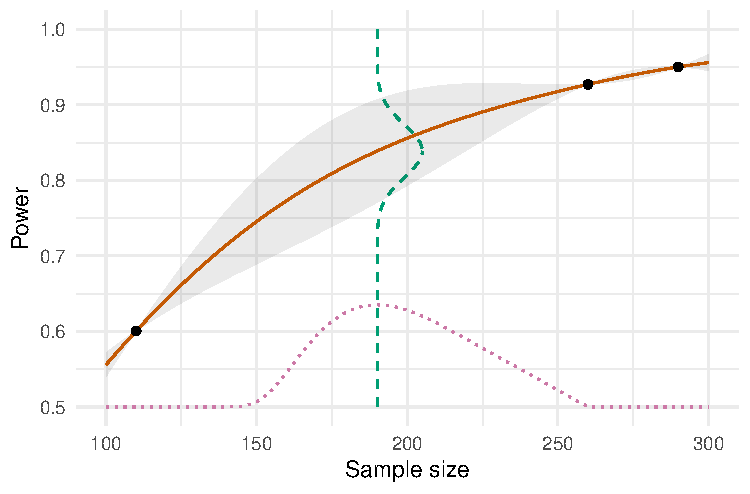
\includegraphics[scale=0.8]{./Figures/GP_example}
\caption{A Gaussian process model of a power function over a one-dimensional sample size (solid line) based on three evaluations. Uncertainty is shown as the shaded area. Expected improvement (dotted line) is maximised at a sample size of 190, where the predicted power is normally distributed around a mean estimate of 0.84 (dashed line).}
\label{fig:GP_example}
\end{figure}

%This optimisation can be assisted by using derivatives, which are available in closed form~\cite{Rasmussen2006}. The calculation of the log marginal likelihood involves the inversion of an $E \times E$ matrix, an operation which requires $\mathcal{O}(E^{3})$ time. In the problems we are interested in $E$ will typically be in the order of hundreds, meaning the calculation of (\ref{eqn:loglik}) is fast and thus the maximum likelihood optimisation remains tractable.

%The optimisation of $\boldsymbol{\theta}$ may involve several local minima, and so there is no guarantee that the solution produced by a numerical optimiser will be the globally optimal solution. It is therefore recommended that the resulting mean function of the conditional distribution over $\mathcal{X}$ is examined graphically to ensure it broadly aligns with prior expectations. Another way to test the quality of the fitted Gaussian process is to predict the value of $f$ at an unobserved point $\mathbf{x}_{*}$, and compute an MC estimate at that point for comparison. This can be done over the course of the efficient global optimisation algorithm (EGO), which we describe in the following section.

\subsubsection{Expected improvement}\label{sec:EGO}

At step (4) in algorithm~\ref{alg:EGO} we consider all solutions $\mathbf{x} \in \mathcal{X}$ and attempt to find that which maximises expected improvement, a measure which we now define. 

%\subsubsection{Simple objective functions}

We first consider the case of expensive constraint functions but cheap and deterministic objective functions, as found in the cross-classified psychotherapy example. We combine multiple objective functions into a single function in the manner proposed in~\cite{Knowles2006}. At each iteration of the algorithm the objective values $f_{i}(\mathbf{x})$ corresponding to objectives $i = 1, \ldots , B$ are first normalised with respect to their limits, leading to values in $[0,1]$. We then calculate a weighted composite objective function
\begin{equation}
f_{\mathbf{w}}(\mathbf{x}) = \sum_{i=1}^{B}w_{i}f_{i}(\mathbf{x}).
\end{equation}\label{eqn:composite}
The vector of weights $\mathbf{w} = (w_{1}, \ldots , w_{B})$ is sampled from a flat Dirichlet distribution at each iteration and so the relative priorities of the search process fluctuate over time, helping to locate a range of solutions offering different trade-offs between the set of objectives. For notational convenience we will drop the subscript $\mathbf{w}$. Denoting the lowest composite objective value obtained by the solutions $\mathcal{X}_{E}$ as $f_{min}$, the improvement which would be obtained by evaluating the solution $\mathbf{x}_{*}$ is simply $f_{min} - f(\mathbf{x}_{*})$.

Any anticipated improvement in the objective $f$ at $\mathbf{x}_{*}$ must be balanced with the probability that the solution will be feasible. Given some MC estimates of an expensive constraint $g$, we can construct a GP model of the function as described in Section~\ref{sec:GP}. The model will give a prediction $g(\mathbf{x}_{*}) \sim \mathcal{N}(m, s^{2})$, and we will consider the point $\mathbf{x}_{*}$ feasible if the upper $p$\% quantile of this distribution is below 0. We denote this quantile as
\begin{equation}
q(\mathbf{x}_{*}) = m + \Phi^{-1}(p)s,
\end{equation}
where $\Phi$ is the standard normal cummulative distribution. Following an evaluation of $\mathbf{x}_{*}$ the GP model will be updated and the quantile revised to $q_{+}(\mathbf{x}_{*})$. Before the evaluation the value of $q_{+}(\mathbf{x}_{*})$ is unknown, but it is shown in~\cite{Picheny2014} that its predictive distribution is $q_{+}(\mathbf{x}_{*}) \sim N(m_{+}, s_{+}^{2})$ where
\begin{align}
m_{+} &= m + \Phi^{-1}(p)\sqrt{\frac{\omega^{2}s^{2}}{\omega^{2} + s^{2}}} \\
s_{+}^{2} &= \frac{[s^{2}]^{2}}{\omega^{2} + s^{2}},
\end{align}
and $\omega$ is the MC error of the planned evaluation. This predictive distribution can be used to calculate the probability that the point $\mathbf{x}_{*}$ will be considered feasible following its evaluation. The improvement in the composite objective function is multiplied by this probability, thus penalising candidate solutions with a low chance of satisfying the constraint~\cite{Sasena2002}. Specifically, we choose to evaluate the solution which maximises
\begin{equation}
EI = [f_{min} - f(\mathbf{x}_{*})] \prod_{j=1}^{C} \Phi\left(\frac{-m_{j,+}}{s_{j,+}}\right),
\end{equation}
where we now include all $j = 1, \ldots , C$ constraint functions.

To illustrate expected improvement we return to the one-dimensional problem illustrated in Figure~\ref{fig:GP_example}. We aim to find a sample size which has power of at least 80\%, with the lowest feasible sample size found so far being 

If we aim to find a sample size which has at least 80\% power, we can see that the mean function of the GP model crosses this threshold at a sample size of 171. However, the expected improvement 

Returning to the one-dimensional example of Figure~\ref{fig:GP_example}, the expected improvement is plotted as a dashed line. We see that although the GP model of the power function suggests that the expected power of a sample size of 171.

%\subsubsection{Expensive objective functions}
%
%We now consider the case where objective functions are not simple deterministic function of the solution and instead require approximation through the MC method (e.g. the expected sample size functions in the multi-arm multi-stage example). As before, multiple objective functions are normalised and combined using a randomly generated weight vector $\mathbf{w}$, but now we are combining estimates $y_{i}$ as opposed to true values $f(\mathbf{x})$. Ignoring subscripts again, at each iteration of the algorithm we then have a vector of estimated composite function values $\mathbf{y} = f(\mathcal{X}_{E}) + \Delta$, where as before $\Delta$ is a diagonal matrix containing the MC errors for each $\mathbf{x} \in \mathcal{X}_{E}$. For simplicity we will assume that the MC error in objective function estimates will be negligible.
%
%A GP model is fitted to the outputs $\mathbf{y}$ of the composite function $f$ at points $\mathcal{X}_{E}$. Denoting the lowest value obtained in $\mathcal{X}_{E}$ as $y_{min}$, we wish to quantify the improvement over $y_{min}$ we can expect to obtain if we evaluate $f$ at $\mathbf{x}_{*}$. According to the GP model, $f(\mathbf{x}_{*}) \sim N(m, s^{2})$. The probability of an improvement by an amount $I$ is therefore
%\begin{equation}
%Pr[ y_{min} - f(\mathbf{x}_{*}) = I] = \frac{1}{\sqrt{2\pi}s} \exp \left[ - \frac{(y_{min} - I - m)^{2}}{2s^{2}} \right].
%\end{equation}
%Taking the expectation of $I$ then gives
%\begin{align}
%\mathbb{E}[I] &= \int_{I=0}^{I=\infty} I \left( \frac{1}{\sqrt{2\pi}s} \exp \left[ - \frac{(y_{min} - I - m)^{2}}{2s^{2}} \right] \right) dI \\
%	&= s[u\Phi(u) + \phi(u)],
%\end{align}
%where $u = (y_{min} - m)/s$ and $\phi$ is the standard normal density~\cite{Jones2001}. Incorporating the probability of constraint violation as before, we choose to evaluate the solution which maximises
%\begin{equation}
%EI = s[u\Phi(u) + \phi(u)] \prod_{j=1}^{C} \Phi\left(\frac{-m_{j,+}}{s_{j,+}}\right).
%\end{equation}

%To discourage the evaluation of solutions which we expect to be infeasible, we follow~\cite{Sasena2002} and multiply the expected improvement in $f$ at the point $\mathbf{x}_{*}$ by the probability that the solution will satisfy the constraint $g$ after its value has been estimated. We consider a solution $\mathbf{x}_{*}$ feasible with respect to the constraint $g$ if we believe
%\begin{equation}
%Pr[ g(\mathbf{x}_{*}) > 0 ] < 0.01.
%\end{equation}
%Note that the suggested tolerance of 0.01 could be adjusted depending on the perceived importance of the constraint. As in the case of the objective function $f$, a Gaussian process model suggests $g(\mathbf{x}_{*}) \sim \mathcal{N}(m, s^{2})$. We would like to quantify the probability that the point $\mathbf{x}_{*}$ will be considered feasible \emph{after} we have computed the estimate $y \approx g(\mathbf{x}_{*})$. Since the updated Gaussian process model will return a prediction of $g(\mathbf{x}_{*}) \sim \mathcal{N}(y, s_{MC}^{2})$, where $s_{MC}^{2} = m(1-m)/N$ is the anticipated MC error, this will be true whenever $y \leq \Phi^{-1}(0.99)s_{MC}$. The predictive distribution of the MC estimate $y$ is $Y \sim \mathcal{N}(m, s^{2} + s_{MC}^{2})$, and so this probability is given by
%\begin{equation}
%\Phi \left( \frac{\Phi^{-1}(0.99)s_{MC} - m}{\sqrt{s^{2} + s_{MC}^{2}}} \right).
%\end{equation}

%We can see that $Z$ is the sum of three normally distributed random variables. Specifically, we start with $X \sim \mathcal{N}(m, s^{2})$, the Gaussian process model prediction of $g(\mathbf{x}_{*})$. An MC estimate with variance $s_{MC}^{2} = m(1-m)/N$ will be distributed as $Y \sim \mathcal{N}(X, s_{MC}^{2}) = \mathcal{N}(m, s^{2}) + N(0, s_{MC}^{2}) = \mathcal{N}(m, s^{2} + s_{MC}^{2})$. This will lead to an updated Gaussian process model prediction of $g(\mathbf{x}_{*}), Z \sim \mathcal{N}(Y, s_{MC}^{2}) = \mathcal{N}(m, s^{2} + s_{MC}^{2}) + \mathcal{N}(0, s_{MC}^{2}) = \mathcal{N}(m, s^{2} + 2s_{MC}^{2})$. Thus, the probability that the point $\mathbf{x}_{*}$ will be considered feasible with respect to constraint $g$ after an MC estimate of $g(\mathbf{x}_{*})$ with $N$ samples is computed is given by 
%\begin{equation}
%\Phi \left( - \frac{m}{\sqrt{s^{2} + 2s_{MC}^{2}}} \right).
%\end{equation}

\subsection{Implementation}

\subsubsection{Algorithm parameters}

We are required to choose the initial set of points to evaluate before commencing with the EGO algorithm. Whilst a thorough evaluation of all options is beyond the scope of this paper, we can  use recommended rules-of-thumb to guide our choice. It has been suggested that 10 points per dimension of the solution space should be included in the set $\mathcal{X}_{E}$, and that between 25 and 50\% of the overall computation budget should be allocated to these initial evaluations~\cite{}. Given a chosen number of points, a space-filling Latin hypercube sample (specifically, a maximin sample) of this size can be generated using the R package lhs~\cite{Carnell2016}. During the iterative portion of the EGO algorithm, we must choose the number of MC samples $N$ used when computing each estimate. This will be highly dependant on the computational burden of the underlying simulation program. We recommend using 1000 samples where possible. The choice of $N$ should account for the fact that, in practice, fitting GP's to more than around 800 points is infeasible~\cite{Chevalier2014}.

%For both objective and constraint functions, we set the number of MC samples in the above calculations to the total computation budget available at that point. So, we choose the next point to evaluate assuming that we will use all our resources to do so. We actually use only a part of the budget, say $N = 1000$, before stopping and checking again if further evaluation is still warranted. This follows the strategy set out in~\cite{Picheny2010} for optimising noisy functions with on-line allocation of resources.

\subsubsection{Regression diagnostics}

The performance of the optimisation algorithm is dependant on the GP models providing a good representation of the underlying functions. It is therefore important that these models are regularly examined to try and identify any poor fits. One approach is to regularly plot the predicted mean function of the GP model in one or two dimensions, centred at the last evaluated point. In the psychotherapy example, we could for instance plot the GP power model as a function of $k$ for fixed $r$ and $n_{2}$, to ensure it is smooth and monotonic increasing (particularly in the area of interest around the nominal value) as we would expect. We can also contrast the predicted function values with the obtained function values at each iteration.

\subsubsection{Programming and interface}

We have chosen to use R to implement the proposed framework, principaly becasue of the availability of robust and efficient R packages for fitting Gaussain process models (DiceKriging~\cite{Roustant2012}) and for global optimisation (rgenoud~\cite{MebaneJr.2011}). Using R also provides flexibility in terms of the user-writen simulation routines by facilitating various complicated analysis procedures, e.g. multilevel modelling through lme4~\cite{Bates2015}. Example R code is provided in the supplementary material. In order to use this code with a new problem, the user must follow a simple interface. Firstly, they must write their own simulation function which takes two arguments. The first argument describes the trial design, i.e. all variables which are to be optimised over. The second argument defines the parameter values for the population model, i.e the hypothesis under which we want to simulate. The function must return a binary value indicating whether or not the null hypothesis was rejected. In addition to this function, the user must define the hypotheses of interest, the nominal error rate constraints, the upper and lower limits of all design variables, and a function which returns a vector of objective function values for any given trial design. Given these components, the example code can be applied without modification to solve the trial design problem.

To summarise, the following objects must be specified:
\begin{itemize}
\item design space: data frame with fields `name', `low', `up' specifying the name and limits of each design variable;
\item parameters: data frame with fields corresponding to each parameter other than those specified in design space, with each row describing a hypothesis to be simulated under;
\item sim trial(design, params): function which takes as arguments a design data frame (with field names corresponding to those of design space) and a params data frame (i.e. one row of parameters), which will simulate data generation and analysis and return a binary variable indicating the resulting stop/go decision;
\item objectives(design): function taking a design data frame as an argument and returning a $B$ dimension vector of objective function values.
\end{itemize}

\section{Application to the examples}\label{sec:illustrate}

\subsection{Cross-classified psychotherapy trial}

\subsubsection{Illustration}

To illustrate the efficient optimisation method we apply it to the cross-classified psychotherapy trial of Section~\ref{sec:CC}. We first translate the details regarding the population model, sampling model and planned analysis into a simulation program in R, which we have provided in the supplementary material. Given the three dimensions of the solution space, we choose a an initial Latin hypercube sample of 30 solutions and estimate the power of each of these using $N = 250$ MC samples. We then apply algorithm~\ref{alg:EGO} using a remaining budget of 22,500 MC samples, using $N = 250$ of these in each iteration. 

The objective space of the problem is illustrated in Figure~\ref{fig:single_run}, which plots the number of therapists $k$ against the total number of patients $n$. Plotted on Figure~\ref{fig:single_run} are three sets of solutions. Firstly, the initial set of 30 points $\mathcal{X}_{E}$ are seen to be evenly spread across the space. The final set of solutions approximating the Pareto front and plotted in black. Finally, all other solutions evaluated at some point during the iteritive phase of the EGO algorithm are plotted in blue.

\begin{figure}
\centering
%\includegraphics[scale=0.8]{./Figures/single_run}
\caption{Objective values of solutions in the initial set $\mathcal{X}_{E}$ (red), subsequent iterations of the algorithm (blue), and those in the final approximation of the Pareto set (black).}
\label{fig:single_run}
\end{figure}

The final set of solutions are described further in Table~\ref{tab:single_run} in terms of their design parameters and the MC estimate of their power. The standard error is estimated using the Normal approximation, i.e. $se = \sqrt{\hat{\beta}(1-\hat{\beta})/250}$. Note that in all but one cases the upper 99\% confidence interval constructed with this standard error exceeds the nominal type II error rate of 0.2. These solutions are nevertheless considered feasible because the Gaussian process model is used to estimate the type II error rates, allowing information to be borrowed from neighbouring evaluations and greater precision to be obtained. For example, at the point $(r, n_{2}, k) = (0.6768232, 549, 7)$ the MC evaluation alone estimates type II error as $0.208 \pm 0.05971712$ (99\% confidence interval) whereas the GP model estimates $0.1883946 \pm 0.0109728$ (99\% credible interval). For comparison we computed a further MC estimate of the type II error of this design using $N = 10,000$ samples, which gave $0.1915 \pm 0.00003601832$ (99\% confidence interval).

\begin{table}
\centering
\begin{tabular}{l l l l l}
\toprule
$r$ & $n_{2}$ & $k$ & $n_{1} + n_{2}$ & $\hat{\beta} \text{ } (se)$ \\
\midrule
0.5638016 & 486 & 40 &  760.0076 & 0.196 (0.02510649) \\
0.6495110 & 468 & 24 &  771.9712 & 0.128 (0.02112969) \\
0.6635676 & 473 & 15 &  786.8675 & 0.156 (0.02294899) \\
0.6695354 & 485 & 13 &  809.7247 & 0.192 (0.02491072) \\
0.6661190 & 513 & 12 &  854.7190 & 0.184 (0.02450665) \\
0.6644832 & 523 & 11 &  870.5247 & 0.156 (0.02294899) \\
0.6695527 & 524 &  9 &  874.8456 & 0.204 (0.02548600) \\
0.6761564 & 543 &  8 &  910.1529 & 0.160 (0.02318620) \\
0.6768232 & 549 &  7 &  920.5759 & 0.208 (0.02566990) \\
0.6909196 & 588 &  6 &  994.2607 & 0.196 (0.02510649) \\
0.8050653 & 864 &  5 & 1559.5764 & 0.168 (0.02364538) \\
\bottomrule
\end{tabular}
\caption{Solutions found by the EGO algorithm with a total budget of 30,000 MC samples.}
\label{tab:single_run}
\end{table}

\subsubsection{Comparison}

We now compare the performance of the efficient optimisation method with the simpler heuristic algorithm described in Section~\ref{sec:CC}. Given the stochastic nature of both algorithms, the comparison is repeated 1000 times. In each instance the heuristic algorithm is applied, using $N$ MC samples for each solution evaluation. The total number of MC samples used over the course of the heuristic is recorded, as is the time taken. The EGO algorithm is then applied, terminating when either the number of MC samples or the time taken equal those used by the heuristic. The EGO algorithm always uses a 30-point Latin hypercube sample as its initial set of solutions $\mathcal{X}_{E}$. The number of MC samples used when evaluating these initial points is set to 25\% of the total budget, or 50 samples per point, whichever is larger. This process is carried out for $N = 100, 250$ and $500$.

We first consider the ability of each method to find at least some feasible solution for each value of $k$. Note that such a solution need not be explicit, in the sense that if a feasible solution for a lower value $k_{*}$ has been found then we can assume that increasing the number of therapists to $k$ whilst keeping all other design variables constant will also be feasible. Across all $k$ and all 1000 runs, the proportions for which no feasible solutions were found are summarised in Table~\ref{tab:missing}. We see see that for each value of $N$ considered, the EGO algorithm has considerably more success in finding feasible solutions than the heuristic. These results are detailed further in Figures~\ref{fig:missing_100},~\ref{fig:missing_250} and~\ref{fig:missing_500}, which illustrate number of times no feasible solution was found for each value of $k$. As we would expect, the lower values of $k$ are the less likely to be obtained.




\subsection{Cluster-randomised pilot trial}

Define the method parameters.

\subsubsection{Illustration}

We illustrate the Bayesian optimisation approach as applied to the cluster randomised pilot trial example of  Section~\ref{sec:examples}. We used a 60-point Latin hypercube sample generated using the maximinLHS function of the lhs package in R as the initial experimental design. MC estimates of power under each hypothesis were computed using $N = 250$ samples. Following this, 60 iterations of Bayesian optimisation were then applied, using $N = 500$ samples for each MC estimate. The resulting approximation set is illustrated in Figure~\ref{fig:pilot_single_run}.

\begin{figure}
\centering
\includegraphics[scale=0.9]{./Figures/pilot_single_run}
\caption{Going up to 60 iterations. We have focussed on the approximation front, omitting 48 points (all from the initial design) which take larger values of $f_{1}$ and/or $f_{2}$. }
\label{fig:pilot_single_run}
\end{figure}

Only 12 of the initial 60 solutions are displayed in Figure~\ref{fig:pilot_single_run}, with the remainder being located outwith the plotted range. The final solutions which form the approximation set are described in further detail in Table~\ref{tab:pilot_single_run}. The results suggests that at least 6 clusters are required in total, given the upper limit of on the number of participants per cluster of 40. Reduction in total number of participants required from 144 to 95 is possible, providing an increase in the number of clusters from 6 to 13 is deemed acceptable. Given the scales involved, an approximation set of size 5 would appear to provide sufficient flexibility for a trial design with the desired balance between objectives to be found.

\begin{table}
\centering
\begin{tabular}{rrrrrrrrrrrrrrrr}
\toprule 
$m_{1}$ & $k_{1}$ & $n_{1}$ & $m_{2}$ & $k_{2}$ & $n_{2}$ & $c_{r}$ & $c_{a}$ & $\hat{\beta} (s.e.)$ & $\hat{\alpha}_{r} (s.e.)$ & 
$\hat{\alpha}_{a} (s.e.)$ & $f_{1}$ & $f_{2}$ \\
\midrule
5 & 7 & 35 & 10 & 6 & 60 & 0.12 & -0.01 & 0.10 (0.01) & 0.29 (0.02) & 0.32 (0.02) & 95 & 13 \\ 
14 & 3 & 42 & 11 & 6 & 66 & 0.12 & -0.01 & 0.10 (0.01) & 0.28 (0.02) & 0.32 (0.02) & 108 & 9 \\ 
16 & 3 & 48 & 13 & 5 & 65 & 0.12 & -0.02 & 0.07 (0.01) & 0.29 (0.02) & 0.35 (0.02) & 113 & 8 \\ 
19 & 3 & 57 & 15 & 4 & 60 & 0.11 & -0.06 & 0.07 (0.01) & 0.28 (0.02) & 0.28 (0.02) & 117 & 7 \\
17 & 3 & 51 & 31 & 3 & 93 & 0.12 & -0.05 & 0.09 (0.01) & 0.28 (0.02) & 0.35 (0.02) & 144 & 6 \\ 
\bottomrule
\end{tabular}
\caption{Solutions in the approximation set following 60 iterations of the Bayesian optimisation algorithm.} 
\label{tab:pilot_single_run}
\end{table}

As can be seen from Table~\ref{tab:pilot_single_run}, approximate upper 99\% confidence limits for the power quantities formed from the original MC estimates often exceed the corresponding nominal bound. For example, the first solution given would have an approximate 98\% two-sided confidence interval of $(0.079, 0.121)$ . However, when the GP model is used to predict power instead of the raw MC estimate, the interval is $(0.082, 0.098)$.  To verify this prediction we computed a more precise MC estimate using $N = 50,000$ samples, giving the interval $(0.091, 0.096)$.

\subsubsection{Comparison}

To compare the two methods described in Section~\ref{sec:methods} we compare the dominated hypervolumes of the resulting approximation sets. In particular, we wish to calculate
\begin{equation}
\Delta = \mathcal{H}(\mathcal{X}_{p}) - \mathcal{H}(A),
\end{equation}
the difference in dominated hypervolumes between the true Pareto set $\mathcal{X}_{p}$ and the attained approximation set $A$. As $\mathcal{X}_{p}$ is unknown, we instead use an approximation generated by repeatedly running the Bayesian optimisation algorithm to obtain $M$ approximation sets $A_{i}, i=1, \ldots, M$ and then finding the set of non-dominated solutions from within the union $\cup_{i=1}^{M} A_{i}$.

Each approximation set $A_{i}$ is obtained through an initial experimental design of 60 points, with $N = 250$ samples used for each MC estimate. This is followed by 200 iterations of Bayesian optimisation using $N = 500$ for each MC estimate. After every 20 iterations the approximation set was found and the difference $\Delta$ calculated. The distributions of these differences as the number of iterations increases is plotted in Figure~\ref{fig:pilot_hv_iters}. For comparison are the results obtained using a fixed experimental design using a Sobol sequence, where the number of solutions included in the design is chosen to lead to a similar computational running time as required by the optimisation algorithm.

\begin{figure}
\centering
\includegraphics[scale=0.9]{./Figures/pilot_hv_iters}
\caption{Boxplots illustrating the differences in dominated hypervolumes obtained as the number of iterations in the Bayesian optimisation algorithm increases. Corresponding differences obtained using the fixed experimental design are shown in red.}
\label{fig:pilot_hv_iters}
\end{figure}

At the start of the iterative portion of the Bayesian optimisation algorithm, Figure~\ref{fig:pilot_hv_iters} shows substantial variability in the quality of the approximation set obtained, with some high quality sets close to the the Pareto front occasionally found already at this point. A random selection of 10 approximation fronts with 0 iterations completed are illustrated in Figure~\ref{fig:pilot_ex_0}.

\begin{figure}
\centering
\includegraphics[scale=0.9]{./Figures/pilot_ex_0}
\caption{Random selection of approximation fronts obtained after 0 iterations of the Bayesian optimisation algorithm (coloured lines), together with the Pareto front (dashed black line) and the approximation front obtained using the fixed experimental design (solid black line).}
% Time taken - 19 mins (on average).
\label{fig:pilot_ex_0}
\end{figure}

The quality of solutions increases substantially as the number of iterations is increased, with the rate of improvement levelling off quite quickly. The updated approximation sets from Figure~\ref{fig:pilot_ex_0} are shown again in Figure~\ref{fig:pilot_ex_60}, now after 60 iterations of the optimisation algorithm. Average quality has clearly increased, although at the cost of computation time - on average, 2 hours and 45 minutes were required to reach 60 iterations, whereas only 19 minutes were needed to evaluate the initial experimental design. However, note that the benefits of the Bayesian optimisation algorithm over the fixed experimental design are clear. As the number of iterations increases to 200, illustrated in Figure~\ref{fig:pilot_ex_200}, the average computation time increases to over 9 hours but the improvement in solution quality is limited.

\begin{figure}
\centering
\includegraphics[scale=0.9]{./Figures/pilot_ex_60}
\caption{Time taken - 2 hrs 45 mins.}
\label{fig:pilot_ex_60}
\end{figure}

\begin{figure}
\centering
\includegraphics[scale=0.9]{./Figures/pilot_ex_200}
\caption{Time taken - 9 hrs 23 mins.}
\label{fig:pilot_ex_200}
\end{figure}



\section{Discussion}\label{sec:discussion}

\begin{itemize}

% strengths, comparison to other methods
\item MLPowSim and SimSam both do simulation based SSD, the former using a very simple grid (although this does lead to a multi-criteria solution of sorts), the latter is limited to problems in one dimension. Note that SimSam could have been used as part of the heuristic algorithm in Example 1 to improve its efficiency. 
\item Many simulation SSD papers already do informal model-assisted design, by getting power at a set of $n$'s and drawing a line through the results.
\item Our approach is very general, can be applied to pretty much any problem as long as we can simulate it and the number of design variables / criteria aren't too large (say, < 10).

% multi-criteria
\item Minimisation of multiple criteria has been discussed for multilevel designs, but always through the \emph{a priori} specification of a weighting function to combine the criteria. We would argue that it will generally be difficult to define such a weighting, that different parties may have different priorities, and that being able to view the exact trade-offs available would often lead to an adjustment of priorities. 
\item Multiple criteria has also been picked up to some extent in the multi-stage adaptive design field, where expected sample size and maximal sample size are often considered. General solution proposed has been to look for `admissible' designs, essentially by solving the problem many times using different weightings in a weighting functions, so very inefficient. Advocated because they can often get a huge reduction in one ciretia at only a small increase in another, so reinforces the point above.

% implementation, applicability, practicality
\item The methods here can be applied fairly easily in R for any proposed simulation, and we can provide the necessary guide to defining the structure and interface of the simulation, and the necessary functions for doing the computations, in an appendix.
\item Just because no analytic solution is available, and simulation must be used, we do not necessarily need the methods here. The MAMS design uses simulation, but the original model is sufficiently simple as to allow very fast simulations. Similarly, in some cases exact solutions are available in the sense that a numerical solver could do the integrations necessary, but the time needed to do so would necessitate the use of the proposed algorithm (although in this case we would have deterministic output).
\item Reproducibility. Don't need to be able to repeat someone's SSD, but do want to be able to confirm the design they propose has the operating characteristics they claim. Will this mean people will have to make their simulation code freely available? If so, would want our software to be easy to use for this purpose. May connect with writing a simulation protocol as described in~\cite{Smith2010}.

% limitations, alternative approaches
\item Could have modelled the penalised objective functions directly, but suspect this may have made the problem much harder to solve as we would be modelling a strange objective function which is very smooth but has a huge, almost discontinuous jump, once a constraint is violated.
\item Modelling all the functions separately assumes independence, when in fact we know there will be correlation. This could potentially be addressed by modelling everything together (`co-krigging'), but this is apparently difficult to do well [RFE], with limited benefits to be gained [REF].
\item Code profiling and efficiency - how much time are we spending getting Monte Carlo estimates, how much time fitting GP models, and how much time optimising the expected improvement criteria? Can any of these be improved? Look at both implementation issues (i.e. writing fast code implementing the proposed algorithm, contrast using R with C / C++, issues around flexibility and transparency~\cite{Smith2010}) and methodological issues (i.e. using better MC algorithms e.g. importance sampling).
\item SSD really involves trading off error rates with sample size, and should be an iterative process. The proposed methods can be used in this manner by simply changing the nominal rates as the search progresses and we get a better picture of the trade-offs involved. We can still make use of all the evaluations made, as opposed to alternative methods which would just start everything again.
\item The proposed optimisation algorithm has a number of parameters which have to be chosen. We have made some suggestions, but for every new problem there will be different optimal choices. Further work and experience in applying the method to a wider range of problems may help in identifying good robust choices for these parameters.
\item We have used GPs, but could consider other non-parametric regression models, e.g. splines, GAMs, etc. Key advantage of GPs is that they provide uncertainty in predictions, so good for sequential optimisation. Key limitation is the scaling with number of points, which in R makes models of more than 200 points quite slow.
\item Could also consider parametric regression models, arguing that the power functions and expected sample size functions may have a form which we could guess at in advance. Although, can always add a model component to the GP and still get the flexibility when modelling the errors.
\item We have focussed, through simulation and non-parametric modelling, on a flexible `black-box' type approach. There may be designs which are very common, yet complex, in which case we may be able to find better solutions tailored specifically to them. 
\item When optimising the improvement criteria, we repeatedly get predictions of the GP models for just one point. We can get predicted values for many points at once with very little extra effort, which suggests a different algorithm which evaluates several points at once may be more efficient.

% extensions
\item Extension to composite hypothesis testing, e.g. when we have nuisance parameters e.g. feasibility parameters around recruitment or correlation parameters for multiple endpoints, which we need to maximise over.
\item Extension to Bayesian SSD, where the simulation will (?) be even more computationally demanding than here.
\item We have worked in R. To help Stata and SAS users make use of this approach, we could try to link the software so that they can write the simulation and analysis in their preferred language and then use an R based routine (GUI?) which calls those simulations.
\item We have only considered frequentist power calculations, but the approach can be applied equally for some Bayesian power equivalent. We have already cited~\cite{Wang2002}, also look at ``SAMPLE SIZE FOR BINOMIAL REGRESSION WITH MISCLASSIFICATION''.
\item We have considered a problem with three error rate constraints, but the method will extend naturally to designs with more e.g. multiple outcome designs with two types of power.
\item For common design problems, rather than everyone optimising to their own local nuisance parameter specification, we could consider building a larger model and holding it centrally for others to use. Analogous to printing sample size tables - we have access to resources here, and could use these to pre-compute and help others without those resources. We would then be interested in a model that gives good predictions, potentially form a very large set of noisy data. So some of the non-parametric machine learning methods mentioned above might be more appropriate.
\item We consider the best solution to be one which has been evaluated, which is a common recommendation. But in the MC setting, it may be that the GP says another point is much better, and we could have it with only a few MC samples. This suggests we could improve through better dynamic allocation of the resources.
\item We have considered deterministic and cheap objective functions only. To tackle trial design problems with stochastic objectives which require simulation to evaluate, e.g. adaptive designs, we need to allow expensive stochastic objectives also.

\end{itemize}

\bibliographystyle{plain}
\bibliography{U:/Literature/Databases/DTWrefs}

\end{document}



















\section{Review}\label{sec:review}

\subsection{Power calculations and sample size determination by simulation}

%\cite{Feiveson2002} - Simple illustrations of how power can be estimated using simulation in Stata. No SSD.

%\cite{Wason2012} - For a MAMS design with a simple model, uses simulation since analytic methods don't work from more than 3 stages. Simulation is simple in the sense that only a multivariate normal test statistic is generated, not individual patient outcome. This is made possible by assuming variance is known - a more realistic model would give the type of computational burden we are interested in. Also, implemented in C so solution method not extendible to other designs. 

%\cite{Burton2006} General review of how simulation studies should be designed, conducted and reported. Not specific to SSD.

%\cite{Smith2010} Similar to Burton et al., a general overview of how a simulation study should be done in accordance with a protocol.

%\cite{Hooper2013} Heuristic algorithm for one dimensional SSD with simulation. Flexible interface, user writes the simulation. Slightly model-based heuristic.

%\cite{Landau2013} General strategy for simulation based SSD. Examples considered only one dimensional.

%\cite{Wang2002} Takes a Bayesian view, notes that we can use MC to evaluate some performance criteria in complex hierarchical models, and then choose the sample size to get the desired level of performance criteria. Only looks at one dimension, discretised. Emphasises the computational burden, meaning the approach may not be that useful in practice. 

%\cite{Baio2015} Focusses on stepped wedge SSD, reviewing some analytical formula and describing how simulation can be used to move past their limitations. The trial designs have three parameters (number of patients, number of clusters, number of observation time points) but only the number of patients is optimised over. Emphasises doing sensitivity analyses for the assumed parameters. Simulates power for some selected values of $n$ and then chooses the lowest which is powered. Suggests around 1000 MC simulations should be enough to estimate power. Includes a comparison of the analytic and simulation methods showing that in some cases the optimal sample sizes are different, so motivating the use of simulation. Has led to an R package "SWSamp"~\cite{} (see also Gianluca Baio's webpage) which uses the algorithm.

%\cite{Grieve2016} Focusses on sample size for logistic regression, and includes the approach of using simulation. Considers one dimensional problems. Starts by describing a bisection search. Then describes the SimSam algorithm. Applies Hooper's algorithm to three case studies.

%\cite{Hooper2016} Focuses on stepped wedge and longitudinal cluster trials. Gives analytical formulae and also described how SimSam can be used, so again only considers a one dimensional problem. Describes as a benefit of formulae over simulation the ability to see the effect of all the parameters - plots the design effect as we vary the cluster size, the ICC and another parameter. Discusses the problems arising from the necessary estimation of the extra parameters coming from these complex designs.

%\cite{Kontopantelis2016} Describes a Stata program ipdpower for sample size in two-level models using simulation, motivated by individual patient level meta-analysis. Mentions SimSam but states that the fact that the data generation model has to be manually specified as a disadvantage - so they are trying to develop something easier to use but less flexible. Doesn't actually do any optimisation, just power calcs, suggest that we can just do a bisection search using these.

%\cite{Schoenfeld2005} Provides an analytic method (an algorithm) for power and SSD for logistic and proportional hazards models. Notes that simulation is an alternative, but at that point too computationally intensive to be practical.

%\cite{Arnold2009} Focussing on the general use of simulation to estimate power, aimed at showing social scientists and epidemiologists who might not be as familiar as statisticians. SSD just by calculating power over a one dimensional range and then plotting. Emphasises the benfits of simulation over its flexibility, particularly that it forces us to be specific about the planned analysis.

%\cite{Shao2007} Group sequential t-tests. Notes that the critical values used in these tests are usually taken from a multivariate normal since the actual multivariate t distribution is too complex to handle. Uses MC estimates of error rates to find the correct critical values empirically. Uses a bisection method when searching for the optimal values.

\subsection{Multi-dimensional sample size calculations}

A common approach to addressing the complexity of multi-dimensional sample size problems is to reduce them to a single dimension. A common example is a trial with a nested, two-level hierarchical structure. Here, the number of patients in each cluster is generally assumed to be fixed in advanced. While this may be appropriate for some cluster randomised studies where clusters are in some sense pre-defined, in other nested trials, such as psychotherapy trials, the size of the cluster may be contollable. Some authors have propsed other one-dimensional variants of the sample size problem in this case, such as where it is the number of clusters which is fixed in advance~\cite{Hemming2011, Eldridge2015}. 



The SSD software MLPowSim~\cite{Browne2009} does allow several-dimension sample size problems relating to multilevel designs to be specified. These problems are solved by specifying a discrete number of values to be used for each parameter.

\cite[p. 175]{Hox2002} - broadly describes how the cost of sampling at each level in a multilevel model should be taken into consideration when choosing sample size. Gives references:

\cite{Snijders1993} - For a two-level nested model, suggests a simple linear cost of sampling at both levels. So treats the problem properly as multi-dimensional, but scalarises objectives to keep it single objective.

\cite{Moerbeek2000} - Considers design issues with multilevel experiments, particularly the level at which we should randomise and the allocation of units at each level. For the latter issue, they first approach the problem of choosing the sample size parameters to minimise the variance in an estimate of a fixed effect, subject to a cost constraint which combines (linearly) the number of units at all levels. This is then extended to find the budget needed to give a desired precision.

\cite{Raudenbush2000} - suggests a linear cost function describing the relative costs of sampling at each of the two levels in a hierarchical model. When might such a function be a realistic characterisation of our preferences? Can we expect to elicit the parametrisation? How sensitive would the results be? Is it generally better to leave the choice to the end? Does it extend well to multiple objectives?

\cite{Breukelen2012} - Considers cluster trials where we can control cluster size. As in~\cite{Moerbeek2000}, starts by defining a cost function relating sampling at the two levels, then finding the sample size that minimises the variance of the fixed effect estimate. The extends to find the sample size needed for some desired power.

\cite{Teerenstra2008} - sample size for three level hierarchial models - clusters, participants, observations. Refers to a cost function proposed in~\cite{Moerbeek2000} to find the best solution given a limited budget.

%\cite{Browne2009} Software for power calcs using MLwiN. Can handle multiple dimensions. Grid search. Not very flexible interface.

%\cite{Hemming2011} - Considers SSD for cluster trials when the number of clusters is fixed, alongside reviewing the usual case when the cluster size is fixed. Also considers the case when both are fixed. Doesn't consider the case when both are free.

%\cite{Eldridge2015} - Designing pilot cluster trials which will estimate an ICC, notes that it is a two dimensional problem but states that often a decision on one of the parameters (cluster size, number of clusters, number of patients) will have been made in advance and so only look at one dimensional problems.

\cite{Sill2012} - Two stage phase II design for two efficacy endpoints. Proposes a simple heuristic method to find the desired design parameters.

\cite{Moineddin2007}

% admissable designs

\cite{Jung2001} - For two stage phase II designs like Simons, with two proposed objectives (expected and maximum sample size), they propose plotting possible designs in the objective space to help people choose something that best reflects their priorities.

\cite{Jung2004} - Following on from~\cite{Jung2001}, they now talk about defining `admissible' designs to be chosen between. They define an artificial loss function which returns either the expected or the maximum sample size depending on if a variable $\omega$ takes the value $\omega_{1}$ or $\omega_{2}$. Then they say this variable has a probability distribution, with probability $q$ for the first and $q-1$ for the second. So now we have an expected loss which is just the linear combination of the two sample sizes with weights $q$ and $q-1$. They then define the Bayes risk as the smallest expected loss over the space of designs, given $q$. So, given some weighting, the `best' design will have the Bayes risk and they call this the Bayes design. An admissible design is one which is a Bayes design. So, there exists a weighting $q$ such that it is the best design. Seems a strange way to go about things - as they show, can lead to efficient designs being classed as inadmissable. Can avoid all this stats/Bayesian language and just use multi-criteria terminology - efficiency, dominated, Pareto.

\cite{Wason2012a} - introduces the $\delta$-minimax design and the corresponding worst case scenario hypothesis. Uses a simple grid search to find optimum designs (in C).

\cite{Wason2011} - Looking just at multistage designs, not multiarm. Takes the criteria from~\cite{Wason2012a} and applies here, introducing a simulated annealing algorithm to find optimal designs since dynamic programming won't work. Compares the optimal designs to alternatives.

\cite{Mander2012} - Extends the~\cite{Jung2004} idea of admissibility to now be a weighted combination of three criteria - expected under null, expected under alternative, and maximum. Describes a way to present results, plotting the weight space and shading areas by the optimal design - doesn't tell us what we are interested in, i.e. how the designs balance the three criteria (admittedly tricky to do so graphically in 3 dimensions). Suggests interpreting the weights in terms of the probabilities of the hypotheses - so a kind of hybrid Bayesianism. To actually find the set of admissable designs, they look at a fine grid over the parameters (which are basically weights in a scalarizing function) and find the corresponding optimal designs - quite inefficient. Only possible because power calculations are analytic for this two stage design. Although in the simulation / simulated annealing work of~\cite{Wason2012} it's said that the admissible idea could easily be applied, it will clearly lead to a massive increase in computational burden.

